\section{Validation Results}
\label{sec:ValidationResults}

\subsection{Trade off Aperture and Power}
\label{sec:PowerApertureTradeoff}

In order to correctly determine the lasing power and the sizing of the receiver aperture, an optimization problem was created. This problem describes how the sizing of both the laser and receiver relate to the total amount of received photons. The method used to solve this problem is the Nelder-Mead (or downhill simplex) method as implemented is the Apache Commons Math library.

The most important parameter is the target amount of photons per pulse per satellite. This reflects the quality of the data. The target is set to 10 photons detected per transmitted pulse, as this will guaranty a decent quality in the BRDF reconstruction. As initial parameters, a power of 5W and an aperture of $10\times10$ cm are used. The performance of each iteration is quantified using the equation \ref{eq:PowerAperturePerformance}:

\begin{equation}
	\text{perf} = \frac {f(\varphi_{total}, \varphi_{target} \times \text{\# sats}, 50) \times 
												\displaystyle\prod_{sat} f(\varphi_{sat}, \varphi_{target}, 200) }
											{ \text{power} \times \text{aperture}^{1.2}}
	\label{eq:PowerAperturePerformance}
\end{equation}

In this equation, f(x, mean, variance) is a normal distribution given mean and variance evaluated at x. A visualization of the results can be seen in figure \ref{fig:PowerAperturePerformance}. It shows the region around the local maximum for the performance function. The results from the optimization algorithm in summary:

\begin{itemize}
	\item Power 4.6W
	\item Aperture 0.0045 m$^2$ (or $6.7\times6.7$ cm)
\end{itemize}

\begin{figure}[ht]
	\centering
	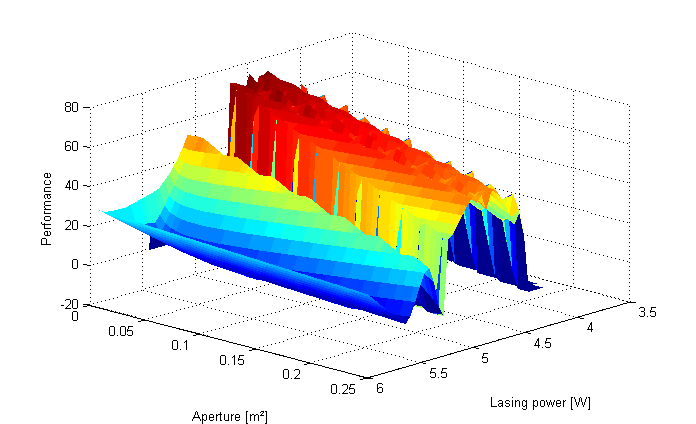
\includegraphics[width=0.6\textwidth]{optimize-PowerAperture.png}%
		\caption{Power-Aperture optimization visualization}%
		\label{fig:PowerAperturePerformance}%
\end{figure}

Note, these results are the bare minimum for the system to operate as designed. When taking a safe margin, this translates into a minimal lasing power of 5.5W and an aperture of 0.0055 m$^2$ ($7.5\times7.5$ cm). 

\subsection{Height Reconstruction}
\label{sec:HeightReconstruction}

The height reconstruction algorithm takes as an input the photons received by the various satellites and the times they were received. Then the photon stream is divided in \emph{interpulse windows}. And interpulse window is as long as one over the pulse frequency. To cut down data volume, the photons inside an interpulse window are divided into a signal window and a noise window. The signal window is centered around the time the signal ought be received (as reconstructed from the emitter history) and bounded by the minimum land elevation (\sim -500 m, for the Dead Sea) and the maximum land elevation (Mt. Everest, \sim 9000 m); any photon that would render another height is not possible on the Earth, and can be discarded directly.

The signal photons are still a pretty mixed lot of noise and actual laser photons, and the next step is to separate the data from the noise. This is done by putting the photons in associated groupings. Before grouping, though, every photon is converted to a height. This is done by constructing an ellipse with the emitter and receiver satellites at the foci, and by setting the angles correctly (from the nadir-pointing requirements) the height is reconstructed.

Then the heights obtained are grouped based on the difference between the altitudes. So for example, if one altitude found is for 50 meters, and the second one is for 50.2 meters, they are recognized as representing the same elevation and grouped together. After the grouping is done, the largest grouping is picked and averaged, and that is the height that is eventually selected. Because the laser photons are much, much more concentrated than the noise photons are, this will filter out the noise and leave us with the data photons; this generally gives a pretty good estimate of the height along the groundtrack.

To improve output quality, further post-processing takes place. The first type of filter used is \emph{spike filtering}. In spike filtering, a data point and the two adjacent heights are compared; if the middle one is more than a certain offset off, it is replaced by the average of the two adjacent points. Another algorithm is \emph{averaging outlier detection}. In this algorithm, a running average is kept, and if the datapoint diverges too much from the average, it is substituted by the average.

When an altitude is substituted, either by the spike or the averaging outlier detection filtering, the program goes through the altitude groupings and looks for the one closest to the average, and takes that one, averages it and substitutes it for the old value. This means that the filters are smarter than they look: they do not just pull data out of the air, but they actually reconsider the signal photons available. This makes the filtering very robust.

For the height determination, accuracies of 3 cm can be obtained when not taking into account sloping, and accuracies of XXXXX IF THIS IS NOT CHANGED TO THE CORRECT VALUE, IT IS ALL SIMON'S FAULT XXXXX cm can be obtained when using the sloping algorithms. 

\subsection{Slope}
\label{sec:Slope}
To facilitate BRDF reconstruction, the slopes are calculated. The along track slope is simply found by averaging the slope over the last few datapoints. The cross track slope is a little more difficult. First the total slope within the footprint is determined based on the height variation within the footprint, found from the different data photons; then the slope is rotated so as to match the along track slope, and then the cross track slope is set so that, when added to the along track slope, it renders the total slope in the footprint.

It is clear that the along track slope can be calculated with greater accuracy and confidence then the cross track slope.

\subsection{BRDF Reconstruction}
\label{sec:BRDFReconstuction}



One on three chance of rain


